\documentclass[11pt, a4paper]{article}
\usepackage{ctex}

\usepackage[margin=1in]{geometry}
\usepackage{color}
\usepackage{clrscode}
\usepackage{amssymb}
\usepackage{amsthm}
\usepackage{amsmath}
\definecolor{bgGray}{RGB}{36, 36, 36}
\usepackage{supertabular}
\usepackage[
  colorlinks,
  linkcolor= blue,
  anchorcolor=blue,
  citecolor=green
]{hyperref}
\usepackage{listings}
\usepackage{fontspec}
\usepackage{graphicx}
\newfontfamily\courier{Courier}
\usepackage{xcolor}

\newcommand{\ilc}{\texttt}

\title{RISC-V CPU report}
\author{冯思远\\516030910575}
\date{}

\begin{document}
\lstset{numbers=left,
  basicstyle=\scriptsize\courier,
  numberstyle=\tiny\courier\color{red!89!green!36!blue!36},
  language=C++,
  breaklines=true,
  keywordstyle=\color{blue!70},commentstyle=\color{red!50!green!50!blue!50},
  morekeywords={},
  stringstyle=\color{purple},
  frame=shadowbox,
  rulesepcolor=\color{red!20!green!20!blue!20}
}
\maketitle
%\tableofcontents
%\newpage

\section{概要}
  这是2017计算机系统(I)大作业的报告文档。项目使用Verilog语言,基于FPGA芯片,实现一个简化的RISC-V指令集CPU。并基于uart通信协议,与PC端的内存系统实现交互。但由于时间较紧,项目未最终完成。如无特殊说明,下文为针对目前进度的报告。
  
\section{计算核心实现}
  项目采用标准五级流水架构,即取指、译码、执行、访存、回写五级流水线。为缓解因RAW产生的stall节拍,增加forwarding操作。分别从执行和访存阶段forwarding到译码阶段。经过优化过后仅当后一条指令对前一条存在数据依赖,且前一条指令为load指令,才会stall一拍,相比原始五级流水有了很大的提升。
\section{内存实现}
  原计划需要将内存实现在pc端,并由uart通信。由于时间原因未达到该程度,现阶段采用模拟内存的方式,并采用uart方式进行通信,尽可能仿真真实情况,并为下一阶段提供经验。内存控制模块采用张哲恺助教的代码,详见\url{https://github.com/sxtyzhangzk/mips-cpu/}

\section{cache实现}
  由于uart通信速度实在太慢,急需cache进行加速。项目采用2路组关联cache,单路采用块大小为16Byte的64行直接映射cache。采用块状读写,即每次读取一整块,即16个Byte。
  \subsection{通信速度}
  根据通信协议,每次读取需要$4*2+5+19=32$个uart周期,而单个读取需要$(4*2+5+5)*4=72$,提速$100\%$以上。即使有$50\%$的数据没有被利用,也比单个读取要快。
  \subsection{块大小}
  经过研究,将块大小定位16Byte,原因如下:(下文提到的周期均为传输一个8bit数据的uart周期)
  \begin{enumerate}
  	\item 由通信速度看,块大小越大,单个数据的平均用时就少。但是这个变化随着块大小的增大而减小。当块大小为32时,平均仍需要1.5个周期,未比块大小16的2周期增加很多。
  	\item 按块读取虽然快,但是如果仅需要少数数据,则会造成大量无效数据的读写。程序有本地性,但是没有本地性的内存,很多情况是仅有一个数据有效,那么造成的代价是$50-18=32$个周期,远大于块大小为16时的$32-18=14$个周期。
  	\item 在cache大小固定的情况下,块大小越大,代表着行数越小,越容易被替换。而替换的代价是很大的,如果被修改过需要2倍于读入的周期。尽可能减少替换可以减少时间。
  \end{enumerate}
  
\section{附录}
	\subsection{架构图}
		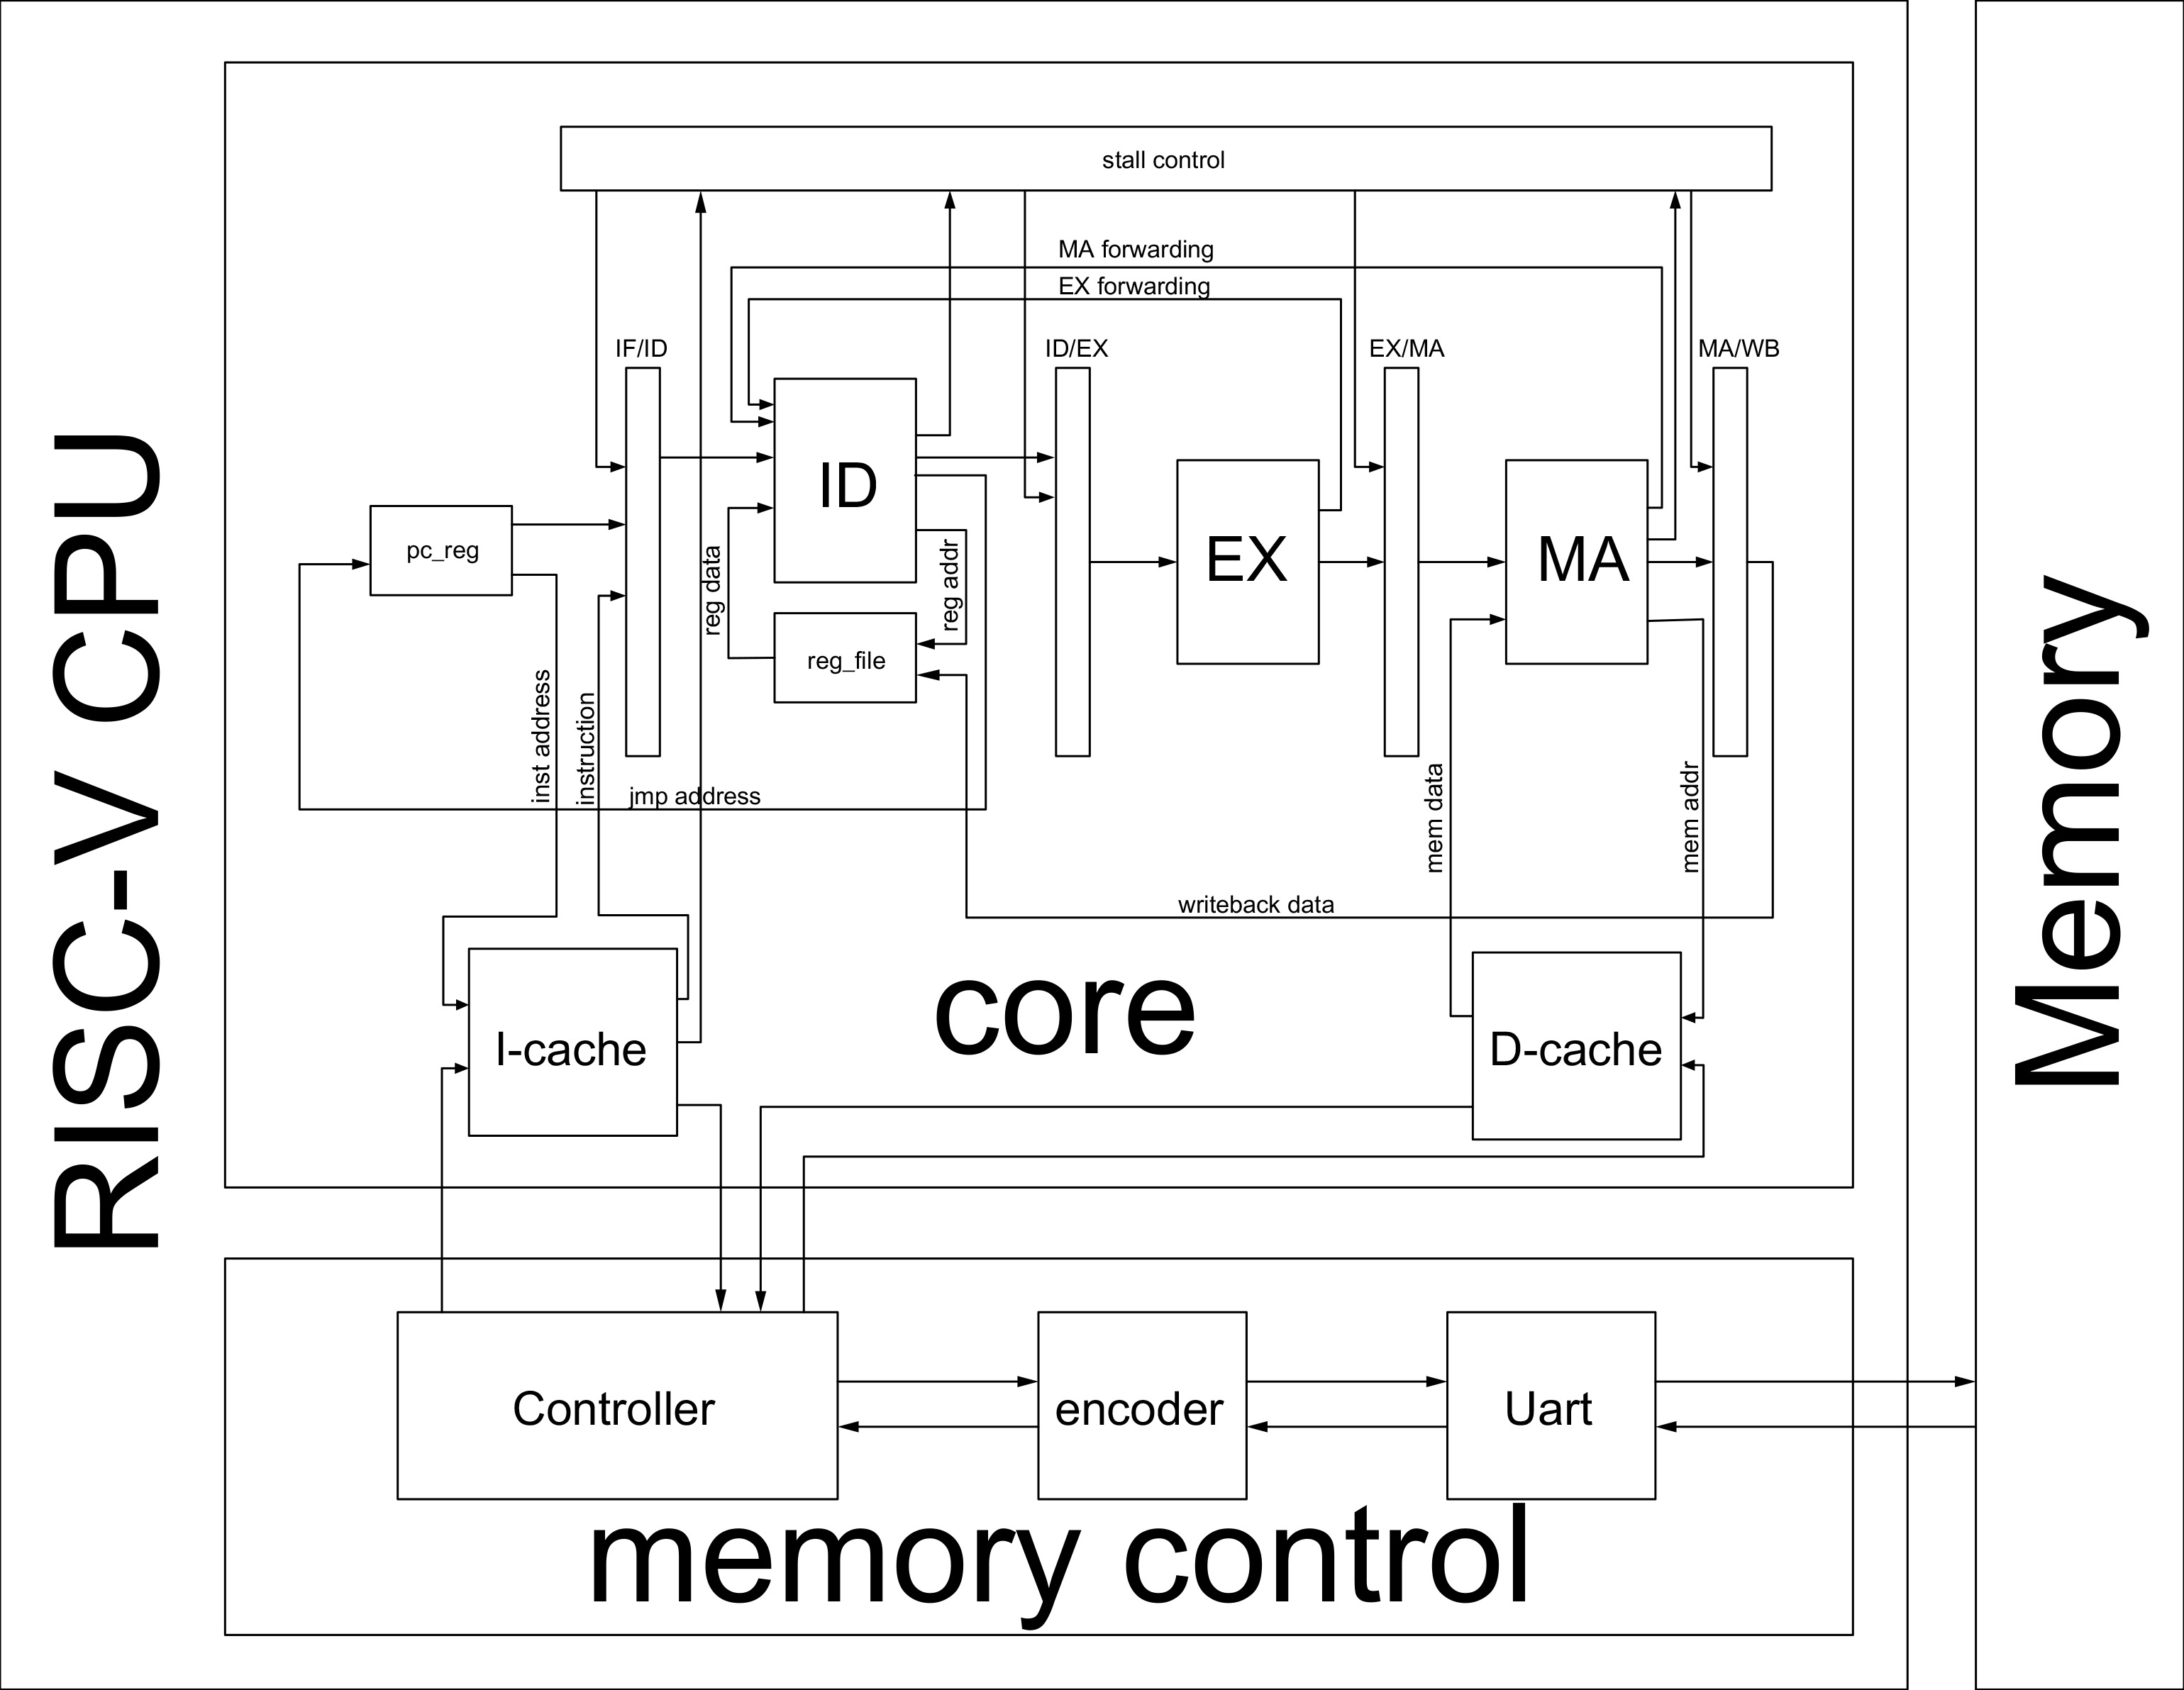
\includegraphics[width=6.5in]{cpu}
	\subsection{参考资料}
		\begin{enumerate}
			\item 助教代码:\url{https://github.com/sxtyzhangzk/mips-cpu/}
			\item 自己动手写CPU(雷思磊, 电子工业出版社)
		\end{enumerate}	
	\subsection{特别感谢}
		提供测试代码的范舟同学和给予我很多帮助的吴章昊同学
\end{document}
